% !TEX TS-program = xelatex
% !TEX encoding = UTF-8 Unicode
% !Mode:: "TeX:UTF-8"

\documentclass{resume}

\usepackage{graphicx}
\usepackage{tabu}
\usepackage{multirow}

\usepackage{zh_CN-Adobefonts_external} % Simplified Chinese Support using external fonts (./fonts/zh_CN-Adobe/)
%\usepackage{zh_CN-Adobefonts_internal} % Simplified Chinese Support using system fonts
\usepackage{linespacing_fix} % disable extra space before next section
\usepackage{cite}

\begin{document}
\pagenumbering{gobble} % suppress displaying page number

\Large{
  \begin{tabu}{ c l r }
  
   \multirow{3}{1in}{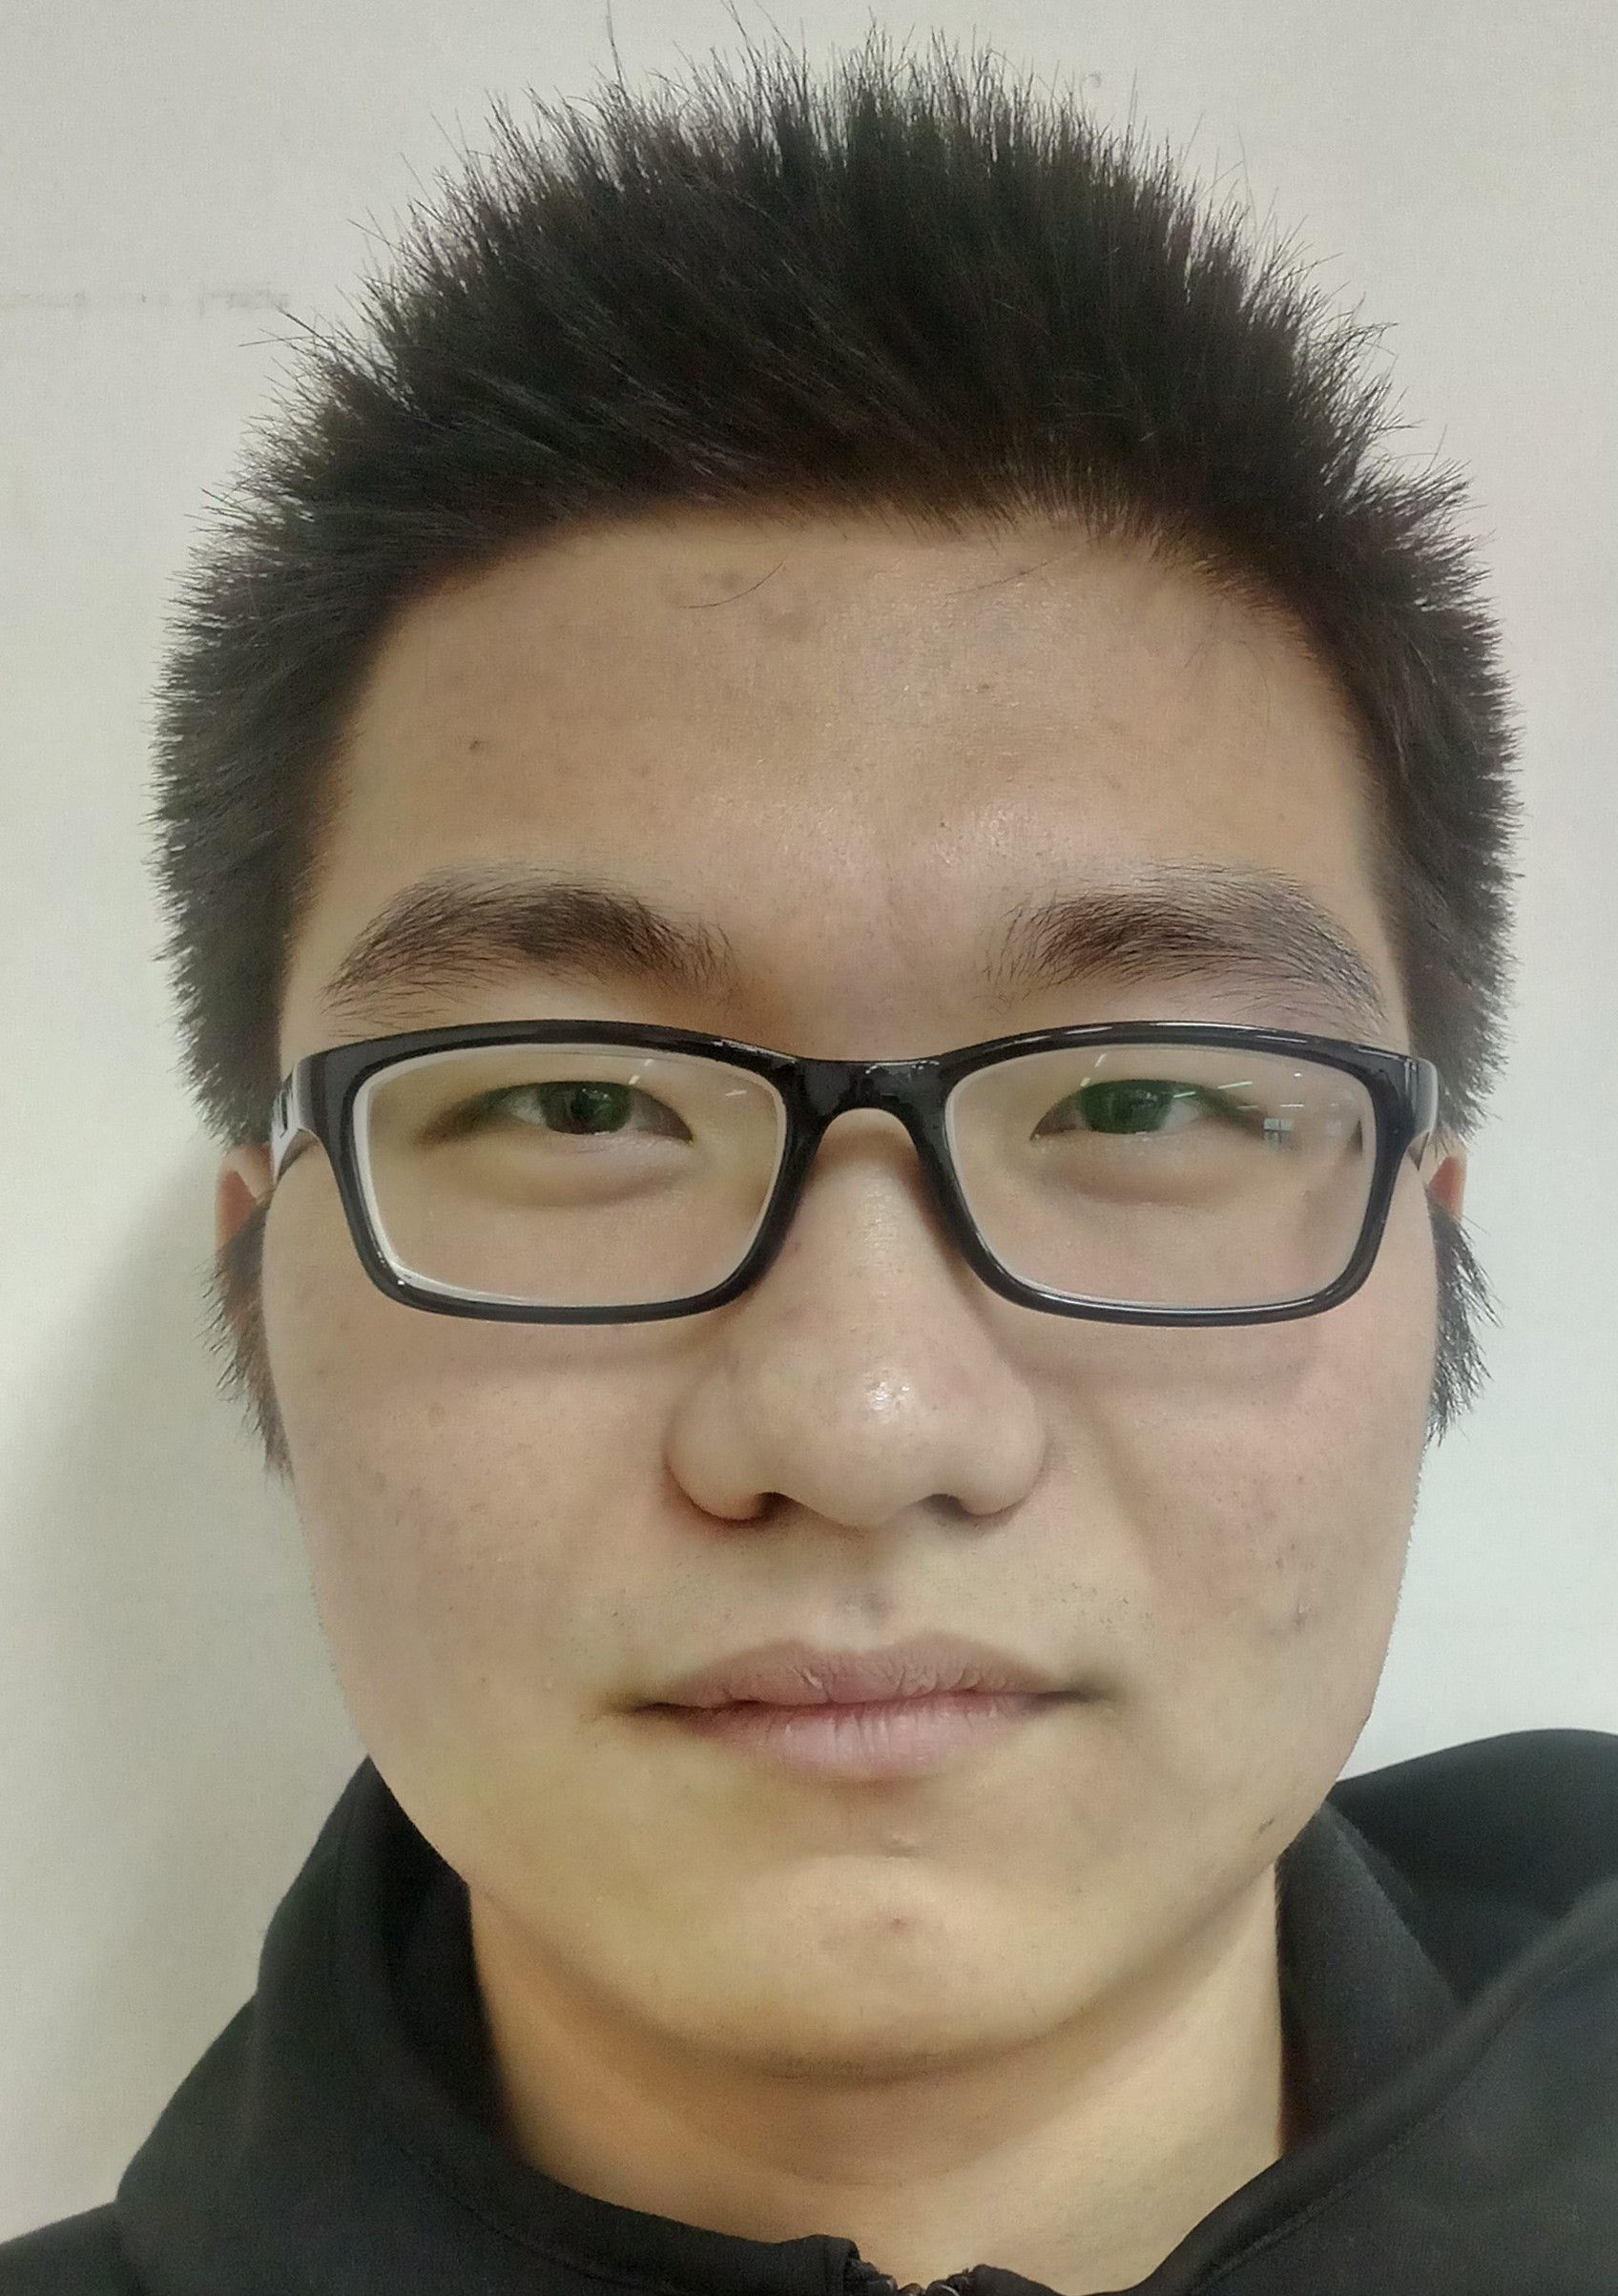
\includegraphics[width=0.88in]{avatar}} & \scshape{徐泽凡} \\
    &\\ 
    & \email{crossoverxzf@qq.com}  \\
    &\\
    & \phone{(+86) 185-0295-1598}
  \end{tabu}
}

\name{徐泽凡}

\basicInfo{
  \email{crossoverxzf@qq.com} \textperiodcentered\ 
  \phone{18502951598} \textperiodcentered
  %\linkedin[billryan8]{https://www.linkedin.com/in/billryan8}
  }
 
\section{\faHeartO\ 求职意向} 
\begin{itemize}[parsep=0.5ex]
  \item Java后端开发实习生
\end{itemize}

\section{\faGraduationCap\  教育背景}
\datedsubsection{\textbf{西安电子科技大学}, 西安, 陕西}{2017.9 -- 至今}
\textit{在读硕士研究生}\   软件工程
\datedsubsection{\textbf{西安电子科技大学}, 西安, 陕西}{2013.8 -- 2017.6}
\textit{学士}\    电子信息工程

\section{\faUsers\ 实习/项目经历}
\datedsubsection{\textbf{黑科技公司} 上海}{2015年3月 -- 2015年5月}
\role{实习}{经理: 高富帅}
xxx后端开发
\begin{itemize}
  \item 实现了 xxx 特性
  \item 后台资源占用率减少8\%
  \item xxx
\end{itemize}

\datedsubsection{\textbf{分布式科学上网姿势}}{2014年6月 -- 至今}
\role{Golang, Linux}{个人项目,和富帅糕合作开发}
\begin{onehalfspacing}
分布式负载均衡科学上网姿势, https://github.com/cyfdecyf/cow
\begin{itemize}
  \item 修复了连接未正常关闭导致文件描述符耗尽的 bug
  \item 使用Chord 哈希 URL, 实现稳定可靠地分流
  \item xxx (尽量使用量化的客观结果)
\end{itemize}
\end{onehalfspacing}

% Reference Test
%\datedsubsection{\textbf{Paper Title\cite{zaharia2012resilient}}}{May. 2015}
%An xxx optimized for xxx\cite{verma2015large}
%\begin{itemize}
%  \item main contribution
%\end{itemize}

\section{\faCogs\ IT 技能}
% increase linespacing [parsep=0.5ex]
\begin{itemize}[parsep=0.5ex]
  \item 编程语言: Java >  C++ == C 
  \item 熟练使用MySQL,Oracle,MongoDB等数据库
  \item 熟悉web开发框架:struts2, hibernate, spring, springMVC, mybatis
  \item 熟悉Linux编程
  \item 英语: CET6,能熟练阅读相关英文文档
\end{itemize}

\section{\faInfo\ 自我评价}
% increase linespacing [parsep=0.5ex]
\begin{itemize}[parsep=0.5ex]
  \item 
  \item 
  \item 
\end{itemize}

%% Reference
%\newpage
%\bibliographystyle{IEEETran}
%\bibliography{mycite}
\end{document}
